\section{Moti Laterali}
I velivoli dotati di ali a freccia positiva, come il Boeing 747, presentano tipicamente un basso smorzamento nei modi laterali.
Tali dinamiche risultano particolarmente difficili da gestire per il pilota, motivo per cui questa tipologia di aeromobili è solitamente equipaggiata con sistemi di controllo automatico volti a supportare e facilitare il lavoro del pilota.

\subsection{Ingressi e Uscite}

I moti laterali oggetto di studio sono influenzati sia dal timone che dagli alettoni. Nel controllo verrà impiegato solamente il timone in quanto ha una maggiore autorità sui moti che si desidera ridurre.

Verrà inoltre utilizzato un giroscopio per misurare l'angolo di imbardata, in quanto particolarmente influenzato dai moti laterali.
\begin{figure}[H]
    \centering
    \begin{tikzpicture}
        \node[draw,
            circle,
            minimum size=0.5cm,
        ] (sum) at (0,0){};

        % Controller
        \node [draw,
            minimum width=2.4cm,
            minimum height=1.2cm,
            right=1.5cm of sum
        ]  (controller) {$Controllore$};

        % System
        \node [draw,
            minimum width=2.4cm,
            minimum height=2.8cm,
            right=1.5cm of controller,
            yshift=0.8cm
        ]  (system) {$Sistema$};

        % Sensor block
        \node [draw,
            minimum width=2.4cm,
            minimum height=1.2cm,
            below right= 1cm and -0.25cm of controller
        ]  (sensor) {$Giroscopio$};


        \draw[-stealth] (system.east) -- ++ (1.5,0)
        node[midway](output){}node[midway,above]{$r$};

        \draw[stealth-] (system.150) -- ++ (-1.5,0)
        node[midway,above]{$\delta_a$};

        \draw[-stealth] (controller.east) -- ++ (1.5,0);

        \draw[-stealth] (sum.east) -- ++ (1.5,0);
        \draw[stealth-] (sum.west) -- ++ (-1.25,0)
        node[midway,above]{$\delta_r$};

        \draw[-stealth] (sensor.west) -| (sum.south);

        \draw[-stealth] (output.center) |- (sensor.east);
    \end{tikzpicture}
\end{figure}

\renewcommand{\arraystretch}{1.2}
\begin{table}[H]
    \begin{tabularx}{\textwidth}{|c|X|}
        \hline
        \multicolumn{2}{|l|}{\textbf{Ingressi}}                                         \\
        \hline
        $\delta_r$ & angolo di deflessione del timone                                   \\
        \hline
        \multicolumn{2}{|l|}{\textbf{Uscite}}                                           \\
        \hline
        $r$        & componente lungo $z_{FRD}$ del vettore $\vec{w}_{FRD}$             \\
        \hline
        \multicolumn{2}{|l|}{\textbf{Variabili di Stato}}                               \\
        \hline
        $p$, $r$   & componenti lungo $x_{FRD}$ e $z_{FRD}$ del vettore $\vec{w}_{FRD}$ \\
        $\beta$    & angolo di derapata                                                 \\
        $\phi$     & angolo di rollio                                                   \\
        \hline
    \end{tabularx}
\end{table}

\subsection{Funzione di Trasferimento}
Utilizzando la funzione \texttt{ss2tf} di MATLAB sul modello di stato \eqref{eq:motoLaterale} si ottiene la funzione di trasferimento:

\begin{equation}
    \label{eq:trasferimentoLaterali}
    \begin{split}
        W_{\delta_r \rightarrow r}(s) & = \frac{-0.475 s^3 - 0.24789 s^2 - 0.11871 s - 0.056462}{s^4 + 0.6358 s^3 + 0.94078 s^2 + 0.51313 s + 0.003683} \\
                                      & = -0.475\frac{(s + 0.4987)(s + 0.0116 \pm j0.4881)}{(s + 0.5630)(s + 0.0073)(s + 0.0328 \pm j0.9478)}
    \end{split}
\end{equation}

Dalla forma di Evans \cite{zampieri_dispensa_controlli}, riportata nella seconda riga, è possibile individuare i poli e gli zeri. In particolare sono presenti tre zeri, $s = -0.4987, s = - 0.0116 \pm j0.4881$, e quattro poli, $s = -0.5630, s = -0.0073, s = -0.0328 \pm j0.9478$

\begin{figure}[H]
    \centering
    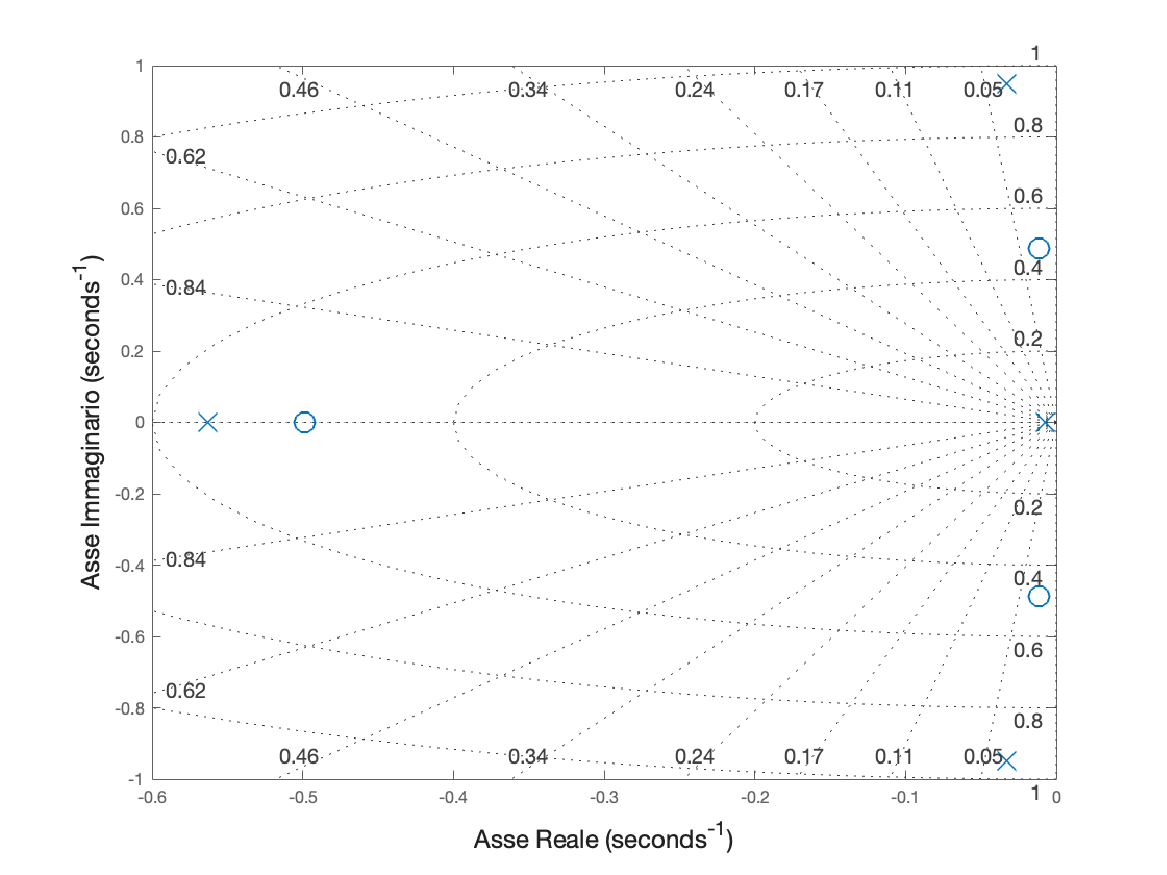
\includegraphics[width=0.7\linewidth]{Immagini/poli_laterali.pdf}
    \caption{\texttt{pzplot} dei poli e degli zeri della funzione di trasferimento $ W_{\delta_r \rightarrow r}(s)$}
\end{figure}

\subsection{Stabilità}

\subsubsection{Stabilità Rispetto alle Condizioni iniziali}

Il polinomio caratteristico del sistema è:
\begin{equation*}
    (s + 0.5630)(s + 0.0073)(s + 0.0328 \pm j0.9478)
\end{equation*}
Le sue radici hanno tutte parte reale $< 0$, è quindi possibile concludere che il sistema è asintoticamente stabile rispetto alle condizioni iniziali.

\subsubsection{BIBO Stabilità}

La funzione di trasferimento ha tutti i poli a parte reale negativa, si conclude che il sistema è BIBO stabile.

\subsection{Modi Naturali}

In questo caso la funzione di trasferimento è costituita da quattro poli: due reali e due complessi coniugati.

I poli reali danno origine a modi criticamente smorzati ($\zeta = 1$), mentre i poli complessi coniugati generano un moto oscillatorio denominato \textit{dutch roll}.

\subsubsection{Spiral}

Il modo associato al polo in $-0.0073$ è detto \textit{spiral}. Esso si manifesta quando, a seguito di una perturbazione, il velivolo acquisisce un angolo di rollio $\phi > 0$.
A seguito della perturbazione la coda del velivolo inizia a generare una componente di portanza, che tende ad aumentare ulteriormente l'angolo $\phi$.

In base all'entità della forza generata, il velivolo può ritornare lentamente alla sua posizione iniziale, come nel caso del Boeing 747, oppure può entrare in una virata di raggio decrescente che può condurre a una pericolosa situazione nota come \textit{graveyard spiral}.

\begin{figure}[H]
    \centering
    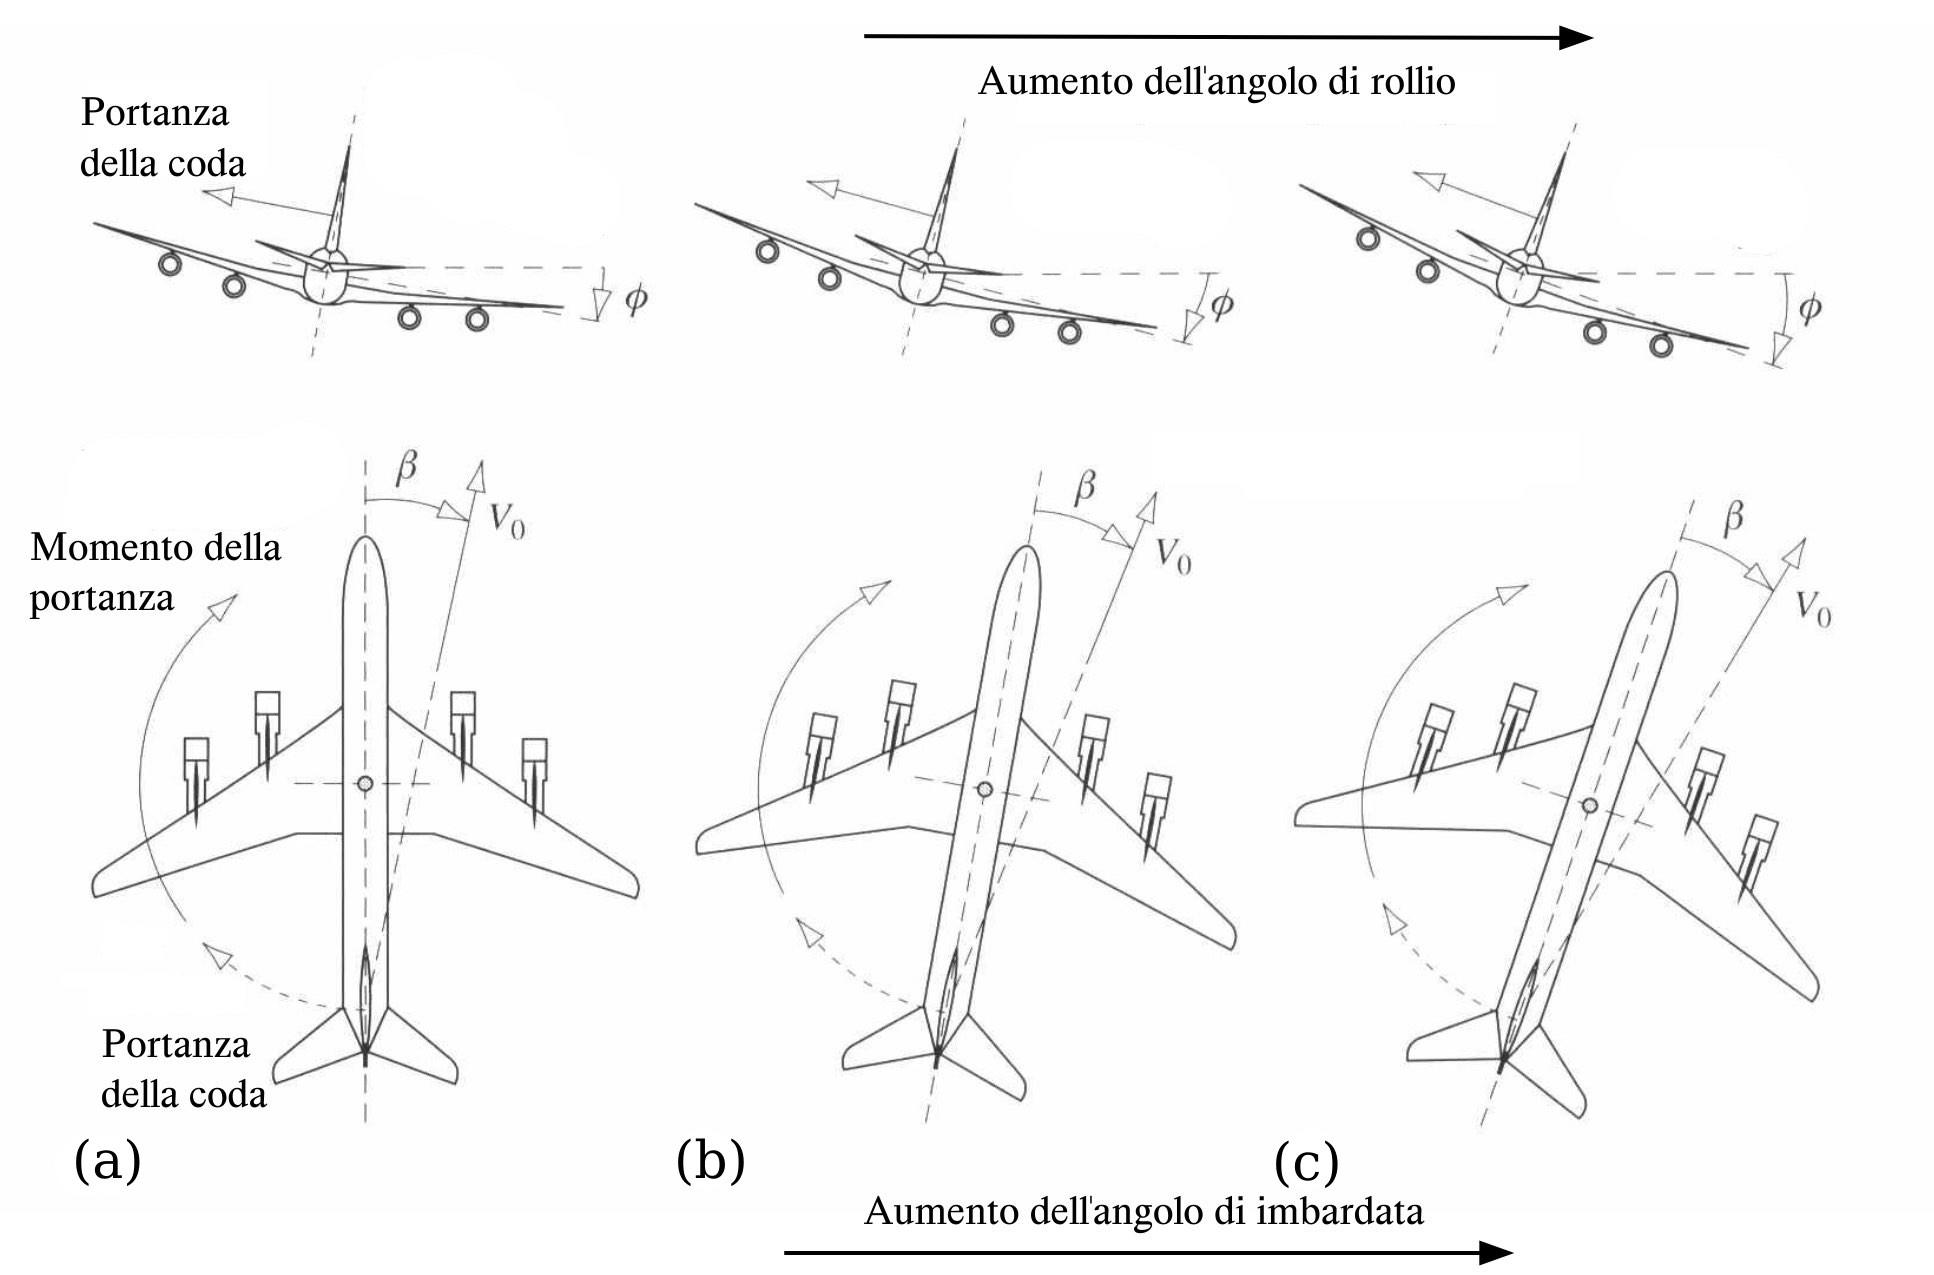
\includegraphics[width=0.8\linewidth]{Immagini/spiral_mode_physics.jpg}
    \caption{Influenza della portanza della coda sull'angolo di rollio e di imbardata \cite{cook1997flight}}
\end{figure}

Dal calcolo del coefficiente di smorzamento e della pulsazione naturale si può osservare come questo modo sia di lungo periodo:
\begin{equation*}
    \zeta = - \frac{Re[p]}{\left|p\right|} = 1 \qquad \omega_n = \left|p\right| = 0.0073rad/s
\end{equation*}

\begin{figure}[H]
    \centering
    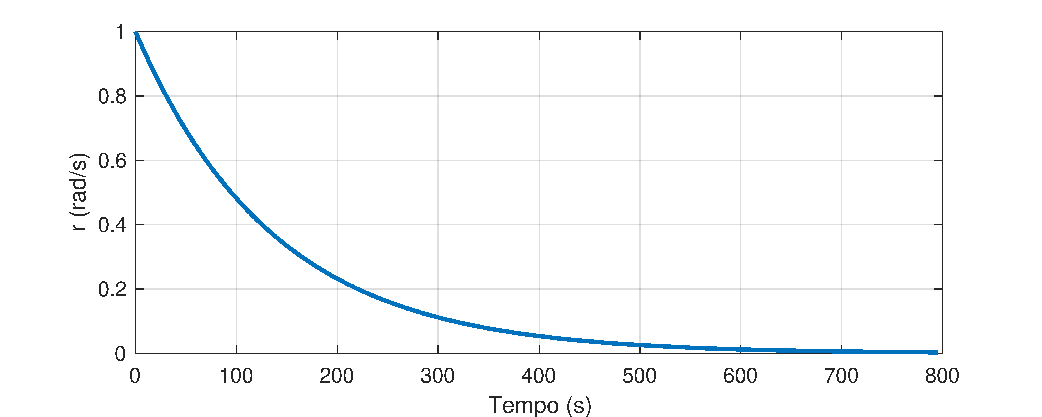
\includegraphics[width=0.7\linewidth]{Immagini/spiral_mode.pdf}
    \caption{Risposta impulsiva per il polo associato al modo \textit{spiral} del Boeing 747 in esame}
\end{figure}

\subsubsection{Roll}

Il modo associato al polo in $-0.5630$ è detto \textit{roll}. Esso si verifica quando il velivolo ruota attorno all'asse $\hat{x}_{FRD}$, ovvero quando la velocità angolare $p$ subisce una variazione.

In questo caso il modo è ben smorzato, quindi il velivolo ritorna rapidamente alla sua condizione di equilibrio dopo una perturbazione.

Ciò è confermato anche dal valore del coefficiente di smorzamento e della pulsazione naturale:
\begin{equation*}
    \zeta = - \frac{Re[p]}{\left|p\right|} = 1 \qquad \omega_n = \left|p\right| = 0.5630rad/s
\end{equation*}

\begin{figure}[H]
    \centering
    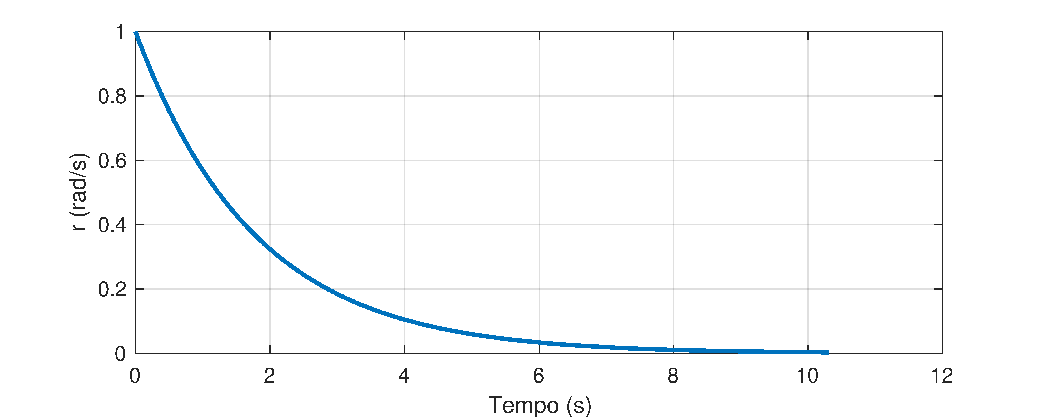
\includegraphics[width=0.7\linewidth]{Immagini/roll_mode.pdf}
    \caption{Risposta impulsiva per il polo associato al modo \textit{roll} del Boeing 747 in esame}
\end{figure}

\subsubsection{Dutch Roll}

Il modo associato ai poli in $-0.0328 \pm j0.9478$ è detto \textit{dutch roll} ed è caratterizzato da un moto oscillatorio che coinvolge simultaneamente rollio, imbardata e derapata.

In particolare, può iniziare con un incremento dell'angolo di imbardata $\psi$, che provoca una variazione dell'incidenza relativa sulle due ali: l'ala avanzata genera una maggiore portanza rispetto all'altra.
Questo squilibrio induce un aumento dell'angolo di rollio $\phi$, che a sua volta altera la direzione del moto e innesca un'imbardata in senso opposto.
Il ciclo si ripete, dando luogo a un'oscillazione di lungo periodo.

\begin{figure}[H]
    \centering
    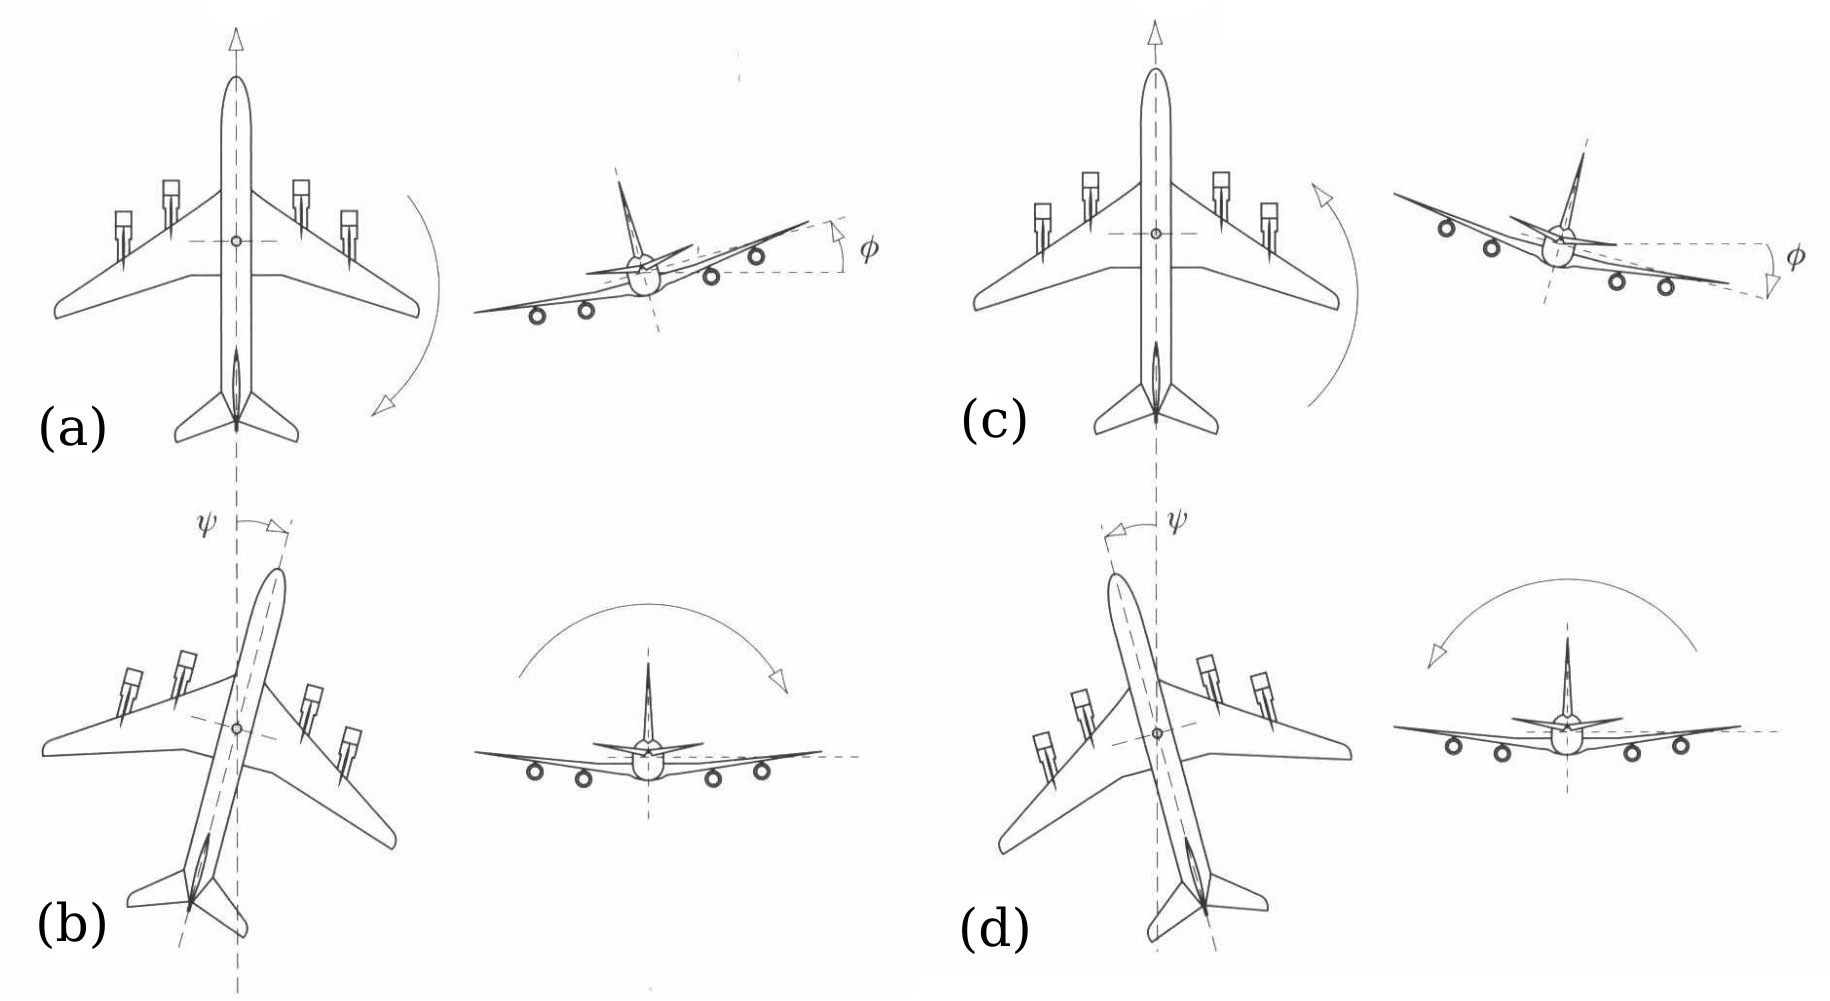
\includegraphics[width=0.8\linewidth]{Immagini/dutch_roll_physics.jpg}
    \caption{Interazione tra gli angoli di rollio e di imbardata \cite{cook1997flight}}
\end{figure}

I parametri del coefficiente di smorzamento e della pulsazione naturale sono:
\begin{equation*}
    \zeta = - \frac{Re[p]}{\left|p\right|} = 0.034585 \qquad \omega_n = \left|p\right| = 0.94836
\end{equation*}

\begin{figure}[H]
    \centering
    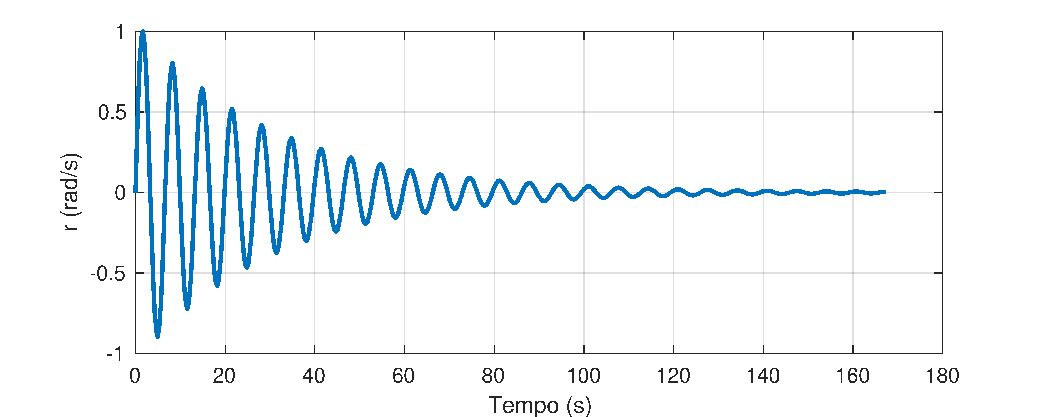
\includegraphics[width=0.7\linewidth]{Immagini/dutch_roll_mode.pdf}
    \caption{Risposta impulsiva per i poli associati al modo \textit{dutch roll} del Boeing 747 in esame}
\end{figure}
